%%%%%%%%%%%%%%%%%%%%%%%%%%%%%%%%%%%%%%%%%
% Beamer Presentation
% LaTeX Template
% Version 1.0 (10/11/12)
%
% This template has been downloaded from:
% http://www.LaTeXTemplates.com
%
% License:
% CC BY-NC-SA 3.0 (http://creativecommons.org/licenses/by-nc-sa/3.0/)
%
%%%%%%%%%%%%%%%%%%%%%%%%%%%%%%%%%%%%%%%%%

%----------------------------------------------------------------------------------------
%	PACKAGES AND THEMES
%----------------------------------------------------------------------------------------

%\documentclass[UTF8,aspectratio=169,14pt]{ctexbeamer}
\documentclass[UTF8,aspectratio=169]{ctexbeamer}
\usepackage{hyperref}
\hypersetup{
	colorlinks=true,
	linkcolor=red,
	anchorcolor=blue,
	citecolor=green
}

\mode<presentation> {
	
	% The Beamer class comes with a number of default slide themes
	% which change the colors and layouts of slides. Below this is a list
	% of all the themes, uncomment each in turn to see what they look like.
	
	%\usetheme{default}
	%\usetheme{AnnArbor}
	%\usetheme{Antibes}
	%\usetheme{Bergen}
	%\usetheme{Berkeley}
	%\usetheme{Berlin}
	%\usetheme{Boadilla}
	%\usetheme{CambridgeUS}
	%\usetheme{Copenhagen}
	%\usetheme{Darmstadt}
	%\usetheme{Dresden}
	%\usetheme{Frankfurt}
	%\usetheme{Goettingen}
	%\usetheme{Hannover}
	%\usetheme{Ilmenau}
	%\usetheme{JuanLesPins}
	%\usetheme{Luebeck}
	\usetheme{Madrid}
	%\usetheme{Malmoe}
	%\usetheme{Marburg}
	%\usetheme{Montpellier}
	%\usetheme{PaloAlto}
	%\usetheme{Pittsburgh}
	%\usetheme{Rochester}
	%\usetheme{Singapore}
	%\usetheme{Szeged}
	%\usetheme{Warsaw}
	
	% As well as themes, the Beamer class has a number of color themes
	% for any slide theme. Uncomment each of these in turn to see how it
	% changes the colors of your current slide theme.
	
	%\usecolortheme{albatross}
	%\usecolortheme{beaver}
	%\usecolortheme{beetle}
	%\usecolortheme{crane}
	%\usecolortheme{dolphin}
	%\usecolortheme{dove}
	%\usecolortheme{fly}
	%\usecolortheme{lily}
	%\usecolortheme{orchid}
	%\usecolortheme{rose}
	%\usecolortheme{seagull}
	%\usecolortheme{seahorse}
	%\usecolortheme{whale}
	%\usecolortheme{wolverine}
	
	%\setbeamertemplate{footline} % To remove the footer line in all slides uncomment this line
	%\setbeamertemplate{footline}[page number] % To replace the footer line in all slides with a simple slide count uncomment this line
	
	%\setbeamertemplate{navigation symbols}{} % To remove the navigation symbols from the bottom of all slides uncomment this line
}

\usepackage{graphicx} % Allows including images
\graphicspath{{./figs/}}
\usepackage{booktabs} % Allows the use of \toprule, \midrule and \bottomrule in tables
\usepackage{longtable}
\usepackage{listings}
\usepackage{xcolor}
\lstset{numbers=left, %设置行号位置
	numberstyle=\tiny, %设置行号大小
	keywordstyle=\color{blue}, %设置关键字颜色
	commentstyle=\color[cmyk]{1,0,1,0}, %设置注释颜色
	frame=single, %设置边框格式
	escapeinside=``, %逃逸字符(1左面的键),用于显示中文
	%breaklines, %自动折行
	extendedchars=false, %解决代码跨页时,章节标题,页眉等汉字不显示的问题
	xleftmargin=2em,xrightmargin=2em, aboveskip=1em, %设置边距
	tabsize=4, %设置tab空格数
	showspaces=false %不显示空格
}
% Fonts
% \usepackage{libertine}
% \setmonofont{Courier}
\setCJKsansfont[ItalicFont=Noto Serif CJK SC Black, BoldFont=Noto Sans CJK SC Black]{Noto Sans CJK SC}
\setmainfont[Ligatures={Common,TeX}]{Linux  Libertine O}
\setmonofont[SmallCapsFont={Latin Modern Mono Caps}]{Latin Modern Mono Light}
\setsansfont{Linux Biolinum O}

\logo{
\includegraphics[width=0.55cm,height=0.55cm]{../../thcs-logo.png}}

%----------------------------------------------------------------------------------------
%	TITLE PAGE
%----------------------------------------------------------------------------------------

\title[第1讲]{第2讲 :OS Architecture \& Structure} % The short title appears at the bottom of every slide, the full title is only on the title page
\subtitle{第四节:Micro kernel -- Mach \& L4 }
\author{陈渝} % Your name
\institute[清华大学] % Your institution as it will appear on the bottom of every slide, may be shorthand to save space
{
	清华大学计算机系 \\ % Your institution for the title page
	\medskip
	\textit{yuchen@tsinghua.edu.cn} % Your email address
}
\date{\today} % Date, can be changed to a custom date


\begin{document}

\begin{frame}
\titlepage % Print the title page as the first slide
\end{frame}

%\begin{frame}
%\frametitle{提纲} % Table of contents slide, comment this block out to remove it
%\tableofcontents % Throughout your presentation, if you choose to use \section{} and \subsection{} commands, these will automatically be printed on this slide as an overview of your presentation
%\end{frame}
%
%%----------------------------------------------------------------------------------------
%%	PRESENTATION SLIDES
%%----------------------------------------------------------------------------------------
%
%%------------------------------------------------
%\section{第一节:课程概述} % Sections can be created in order to organize your presentation into discrete blocks, all sections and subsections are automatically printed in the table of contents as an overview of the talk
%%------------------------------------------------

%-------------------------------------------------
\begin{frame}[plain]
	\frametitle{What is a Microkernel?}
	
	
	
	\begin{columns}
		
		\begin{column}{.4\textwidth}
			
			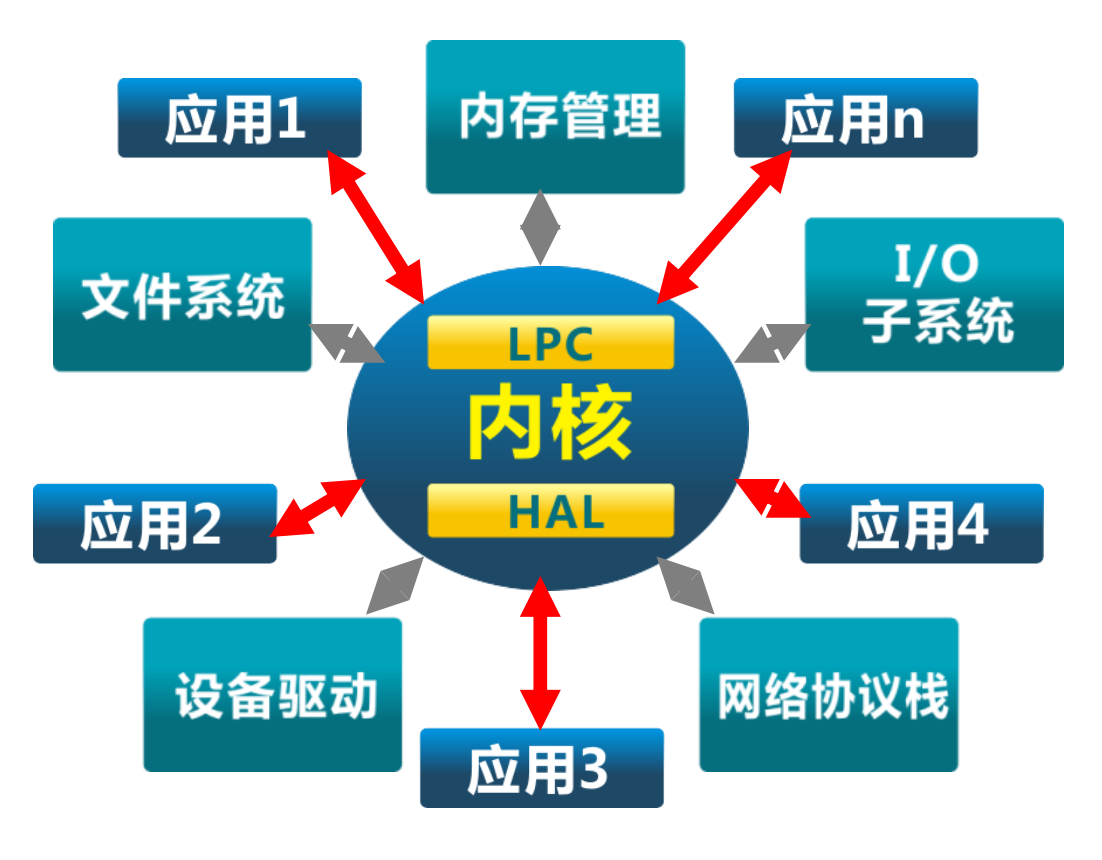
\includegraphics[width=1.\textwidth]{microkernel-arch}
			
		\end{column}
		
		\begin{column}{.6\textwidth}
			
%			\Large
		\begin{itemize}
		\item Kernel with minimal features
		\item Moves as much from the kernel into user space
			\begin{itemize}
				\item Address spaces
				\item Interprocess communication (IPC)
		 		\item Scheduling

		 	
			\end{itemize}	
		\end{itemize}	
%			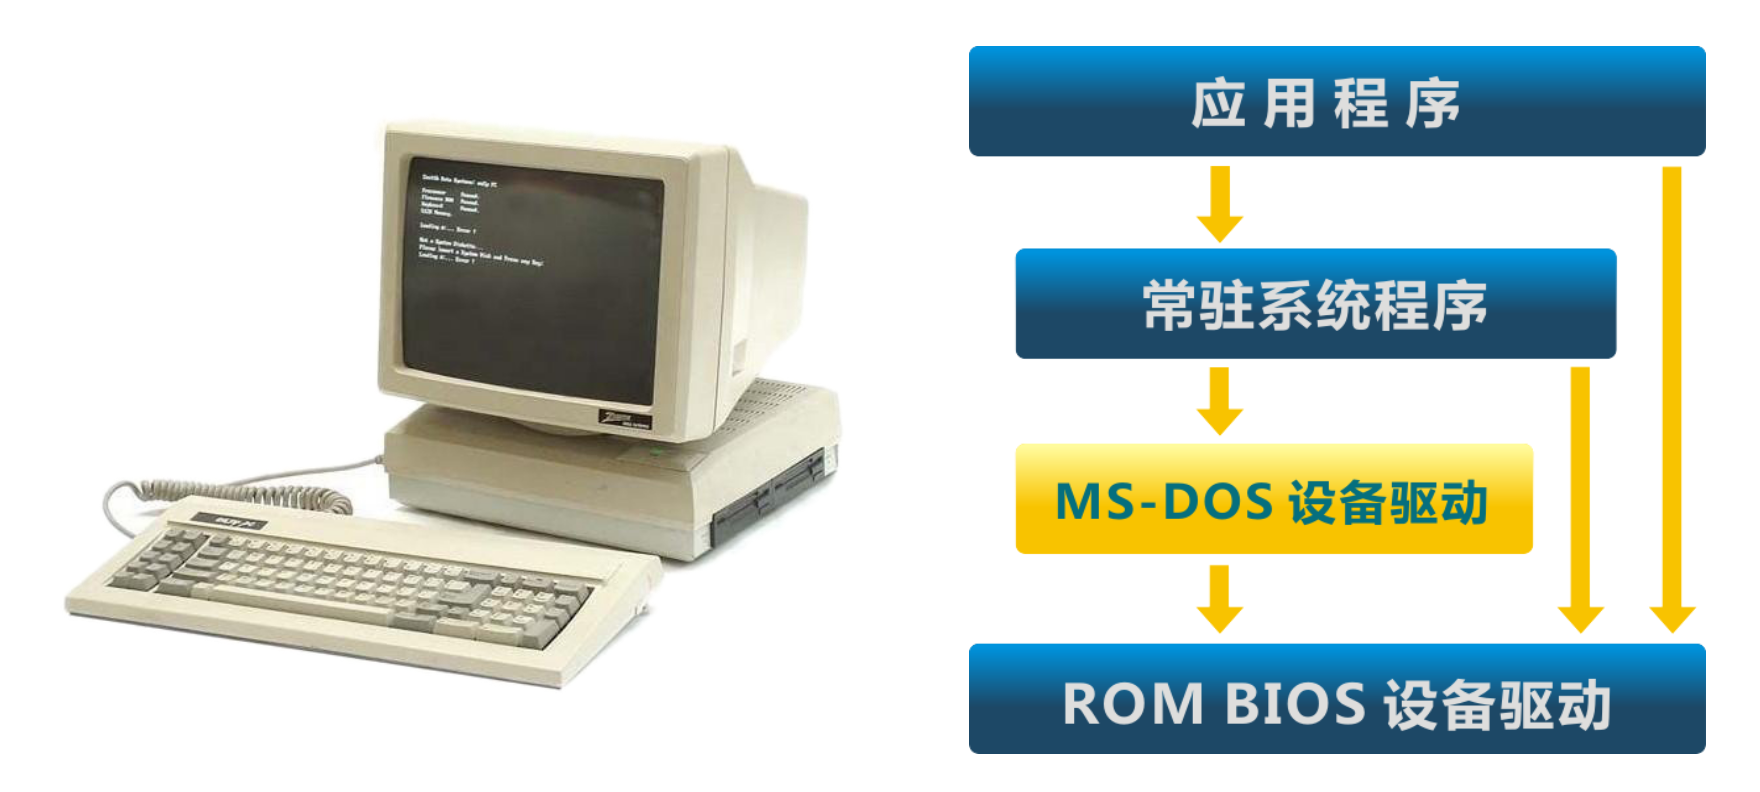
\includegraphics[width=1.\textwidth]{msdos}		
		\end{column}
		
		
	\end{columns}
	
\end{frame}


%-------------------------------------------------
\begin{frame}[plain]
	\frametitle{What is a Microkernel?}
	
	
	
	\begin{columns}
		
		\begin{column}{.5\textwidth}
			
			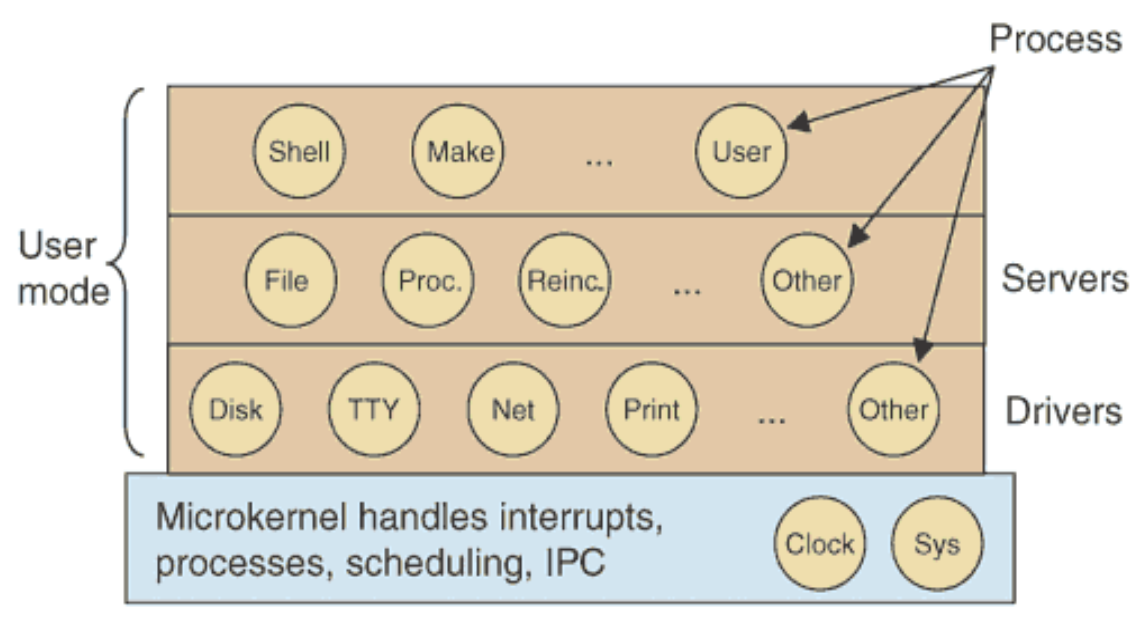
\includegraphics[width=1.\textwidth]{minix3}
			
		\end{column}
		
		\begin{column}{.5\textwidth}
			
			%			\Large
			\begin{itemize}
				\item Benefits

				\begin{itemize}
					\item Flexibility
%					can implement competing versions of key OS features, like filesystem or paging, for best performance with applications.
					\item Safety
%					server malfunction restricted to that server (even drivers), not affecting rest of OS.
					\item Modularity
%					fewer interdepencies and a smaller trusted computing base (TCB).
					
				\end{itemize}	
			
				\item Detriments
				\begin{itemize}
					\item Address spaces
					\item Interprocess communication (IPC)
					\item Scheduling
					
					
				\end{itemize}	
		
			\end{itemize}	
			%			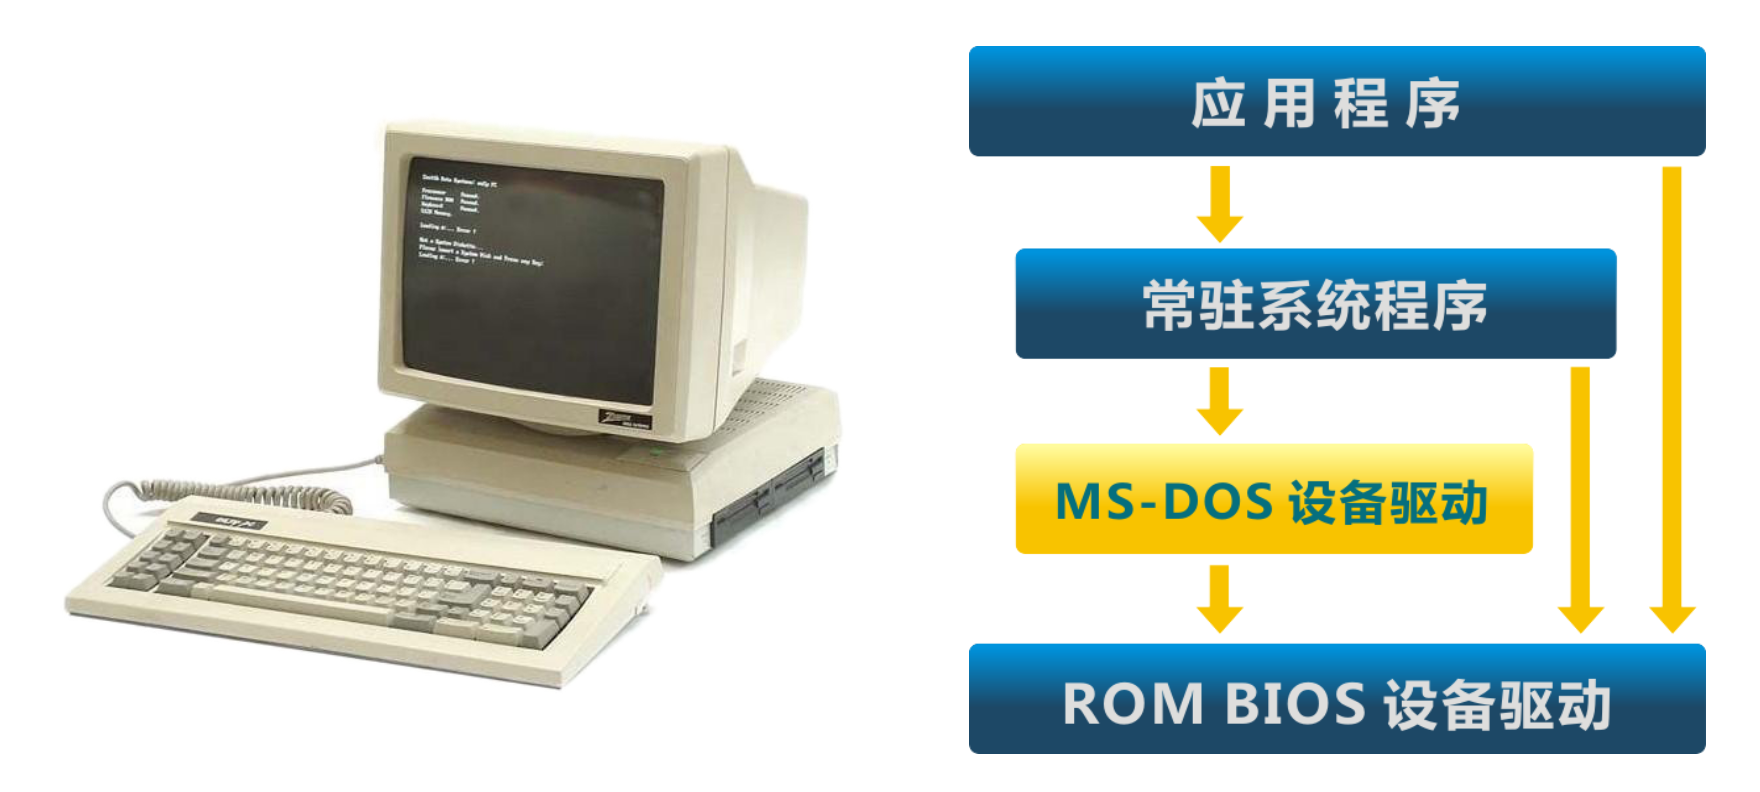
\includegraphics[width=1.\textwidth]{msdos}		
		\end{column}
		
		
	\end{columns}
	
\end{frame}


%-------------------------------------------------
\begin{frame}[plain]
	\frametitle{Microkernel-- Mach}

Mach Developed  at CMU
Led by Rick Rashid, Founded Microsoft Research
Initial  release: 1985

	
%Task: unit of execution consisting of an address space, ports, and threads.
%Thread: basic unit of execution, shares address space, ports with other threads in task.
%Port: communication channel used to send messages between tasks.  Tasks must have correct port rights to send message to a task.
%Message: basic unit of communication consisting of a typed set of data objects.
%Memory Object: source of memory tasks can map into their address space; includes files and pipes.	
	
	\begin{columns}
		
		\begin{column}{.4\textwidth}
			\centering
			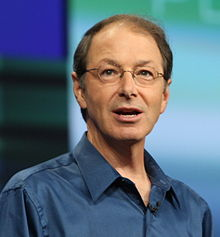
\includegraphics[width=.3\textwidth]{Rick-Rashid}
			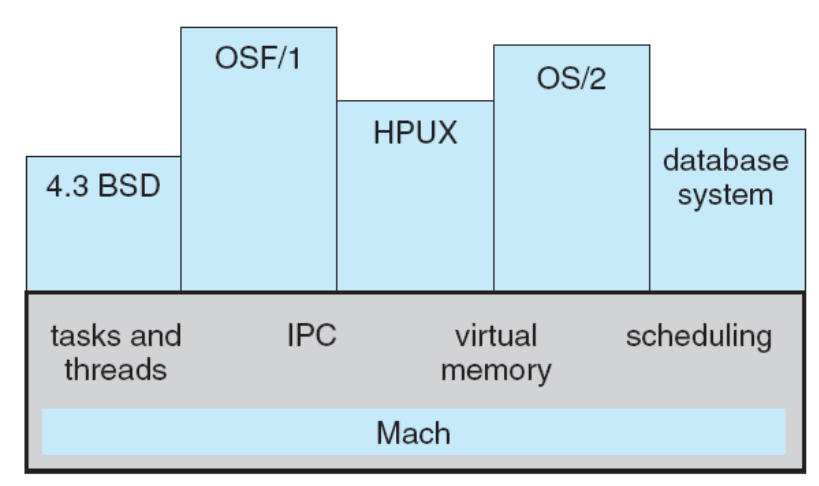
\includegraphics[width=1.\textwidth]{mach-arch}
%			Developed at CMU, Led by Rick Rashid, Initial release: 1985, Big impact (as we will see)
		\end{column}
		
		\begin{column}{.6\textwidth}
			
			%			\Large
			\begin{itemize}
				\item First generation microkernel -- Mach (led by Rick Rashid)
				\item Task and thread management
				\begin{itemize}
					\item Task (process) unit of allocation
					\item Thread, unit of execution
					\item CPU scheduling policies exposed to apps
				\end{itemize}	
				\item Interprocess communication (IPC)
				\begin{itemize}
					\item Between threads via ports
					\item Secured by capabilities

				\end{itemize}				
				
				\item Memory object management
				\begin{itemize}
					\item virtual memory
					\item memory object
					\item hierarchical pagers
					
				\end{itemize}		
			\end{itemize}	
	
		\end{column}
		
		
	\end{columns}
	
\end{frame}


%-------------------------------------------------
\begin{frame}[plain]
	\frametitle{Microkernel-- Mach}
	
	%Task: unit of execution consisting of an address space, ports, and threads.
	%Thread: basic unit of execution, shares address space, ports with other threads in task.
	%Port: communication channel used to send messages between tasks.  Tasks must have correct port rights to send message to a task.
	%Message: basic unit of communication consisting of a typed set of data objects.
	%Memory Object: source of memory tasks can map into their address space; includes files and pipes.	
	
	\begin{columns}
		
		\begin{column}{.4\textwidth}
			\centering
			%			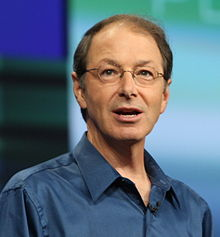
\includegraphics[width=.3\textwidth]{Rick-Rashid}
			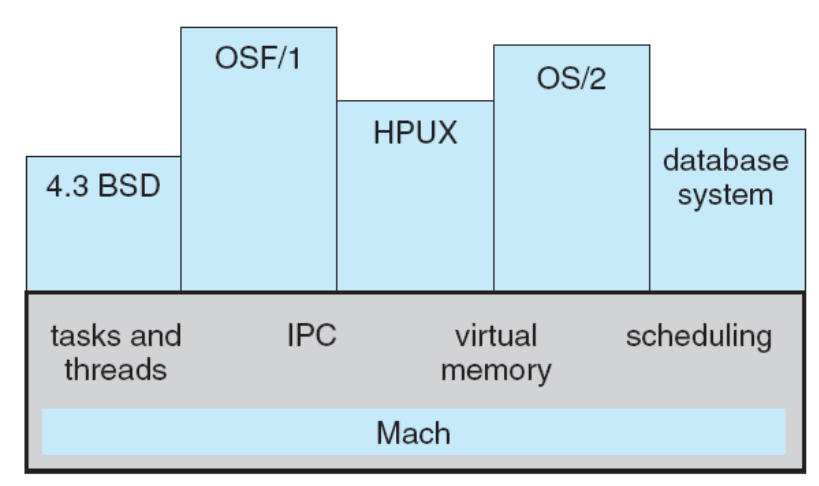
\includegraphics[width=1.\textwidth]{mach-arch}
			%			Developed at CMU, Led by Rick Rashid, Initial release: 1985, Big impact (as we will see)
		\end{column}
		
		\begin{column}{.6\textwidth}
			
			%			\Large
			\begin{itemize}
				\item First generation microkernel -- Mach 
				
			\end{itemize}	
			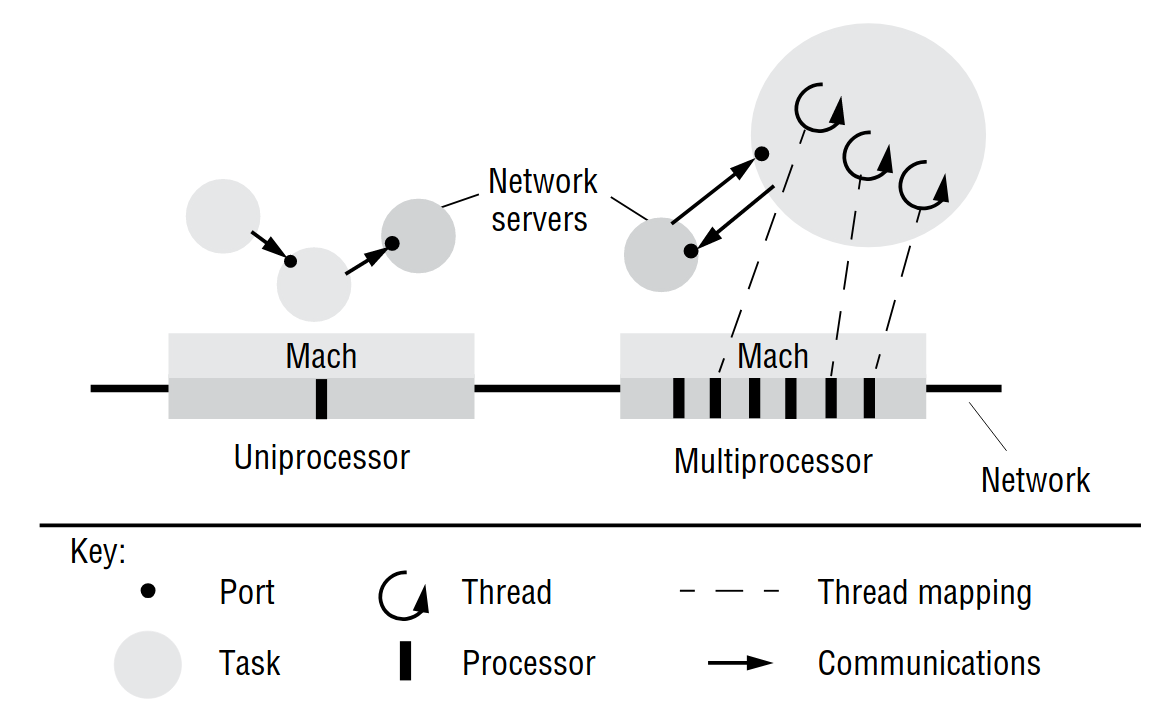
\includegraphics[width=1.\textwidth]{mach-abstract}	
		\end{column}
		
		
	\end{columns}
	
\end{frame}

%-------------------------------------------------
\begin{frame}[plain]
	\frametitle{Microkernel-- Mach}
	
	%Task: unit of execution consisting of an address space, ports, and threads.
	%Thread: basic unit of execution, shares address space, ports with other threads in task.
	%Port: communication channel used to send messages between tasks.  Tasks must have correct port rights to send message to a task.
	%Message: basic unit of communication consisting of a typed set of data objects.
	%Memory Object: source of memory tasks can map into their address space; includes files and pipes.	
	
	\begin{columns}
		
		\begin{column}{.4\textwidth}
			\centering
%			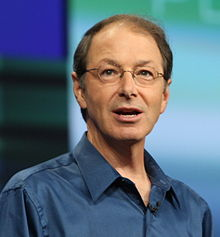
\includegraphics[width=.3\textwidth]{Rick-Rashid}
			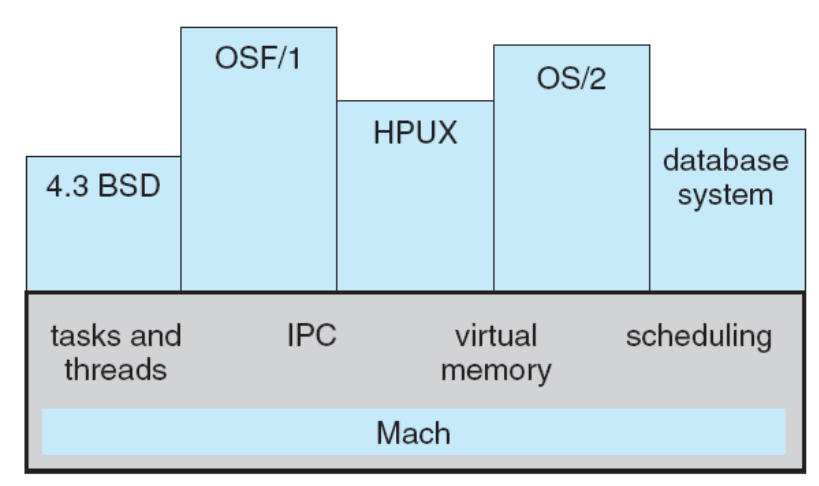
\includegraphics[width=1.\textwidth]{mach-arch}
			%			Developed at CMU, Led by Rick Rashid, Initial release: 1985, Big impact (as we will see)
		\end{column}
		
		\begin{column}{.6\textwidth}
			
			%			\Large
			\begin{itemize}
				\item First generation microkernel -- Mach 
				\item Performance
				\begin{itemize}
					\item the use of IPC for almost all tasks turned out to have serious performance impact. 
					\item system calls take 5-6X as long as UNIX
					\item  given a syscall that does nothing, a full round-trip under BSD would require about 40μs, whereas on a user-space Mach system it would take just under 500μs. 

					\item benchmarks on 1997 hardware showed that Mach 3.0-based UNIX single-server implementations were about 50\% slower than native UNIX.
				\end{itemize}		
			\end{itemize}	
			
		\end{column}
		
		
	\end{columns}
	
\end{frame}




%-------------------------------------------------
\begin{frame}[plain]
	\frametitle{Microkernel-- L4}
	
	%Task: unit of execution consisting of an address space, ports, and threads.
	%Thread: basic unit of execution, shares address space, ports with other threads in task.
	%Port: communication channel used to send messages between tasks.  Tasks must have correct port rights to send message to a task.
	%Message: basic unit of communication consisting of a typed set of data objects.
	%Memory Object: source of memory tasks can map into their address space; includes files and pipes.	
	
	\begin{columns}
		
		\begin{column}{.4\textwidth}
			\centering
			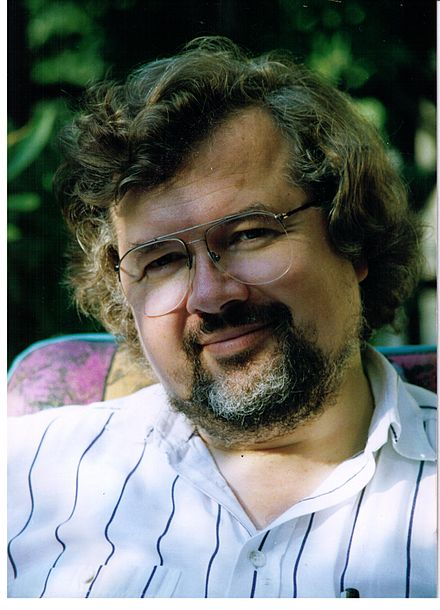
\includegraphics[width=.3\textwidth]{l4-author}
			\\
			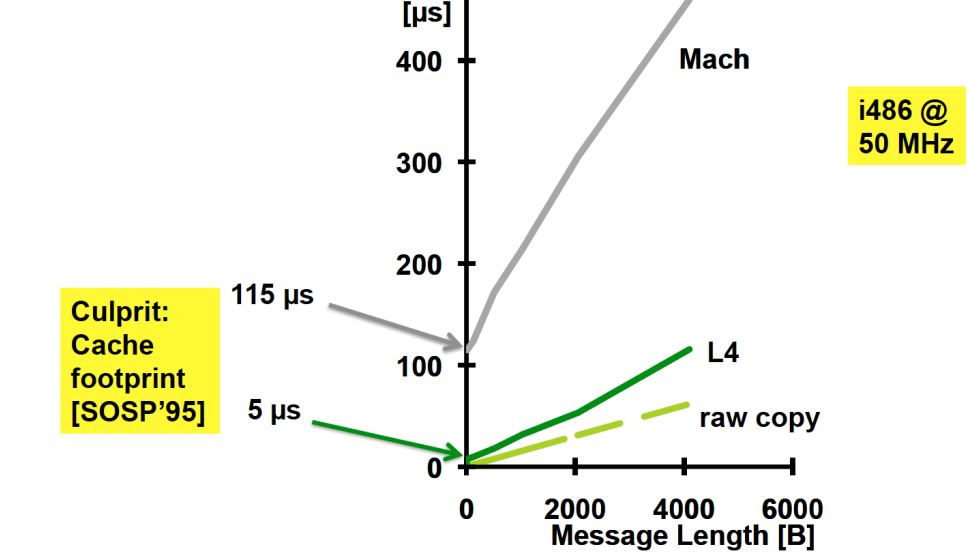
\includegraphics[width=1.\textwidth]{l4-perf}
			%			Developed at CMU, Led by Rick Rashid, Initial release: 1985, Big impact (as we will see)
		\end{column}
		
		\begin{column}{.6\textwidth}
			
			%			\Large
			\begin{itemize}
				\item Second generation microkernel -- L4 by Jochen Liedtke (GMD)
				\item Performance
				\begin{itemize}
					\item synchronous IPCs  -->  async IPCs (like epoll in Linux)
					\item smaller, Mach 3(330 KB) --> L4 (12KB)
					\item IPC security checks moved to user process
					\item IPC is hardware dependent
				\end{itemize}		
			\end{itemize}	
			
		\end{column}
		
		
	\end{columns}
	
\end{frame}


%-------------------------------------------------
\begin{frame}[plain]
	\frametitle{L4 family}
	
	\centering
	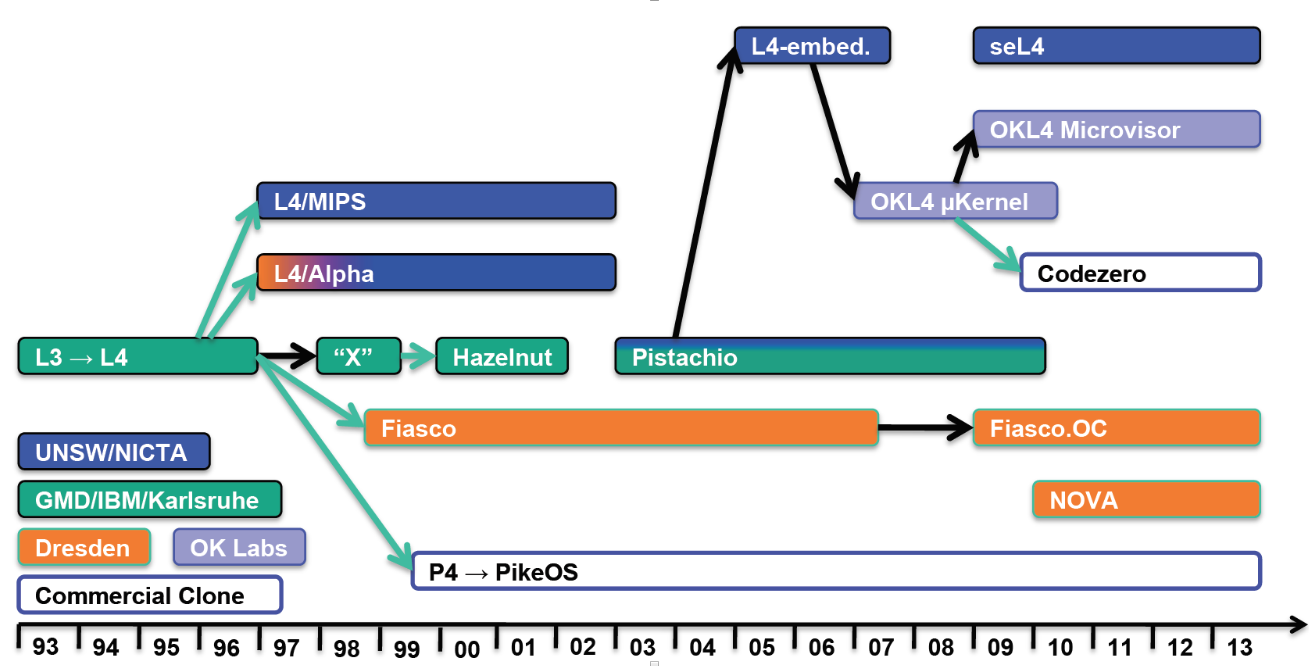
\includegraphics[width=1.\textwidth]{l4-family}
	
\end{frame}



%https://ucbrise.github.io/cs262a-spring2018/notes/18-microkerenels-Mach-seL4.pdf
%-------------------------------------------------
\begin{frame}[plain]
	\frametitle{L4 family}
	
	\centering
	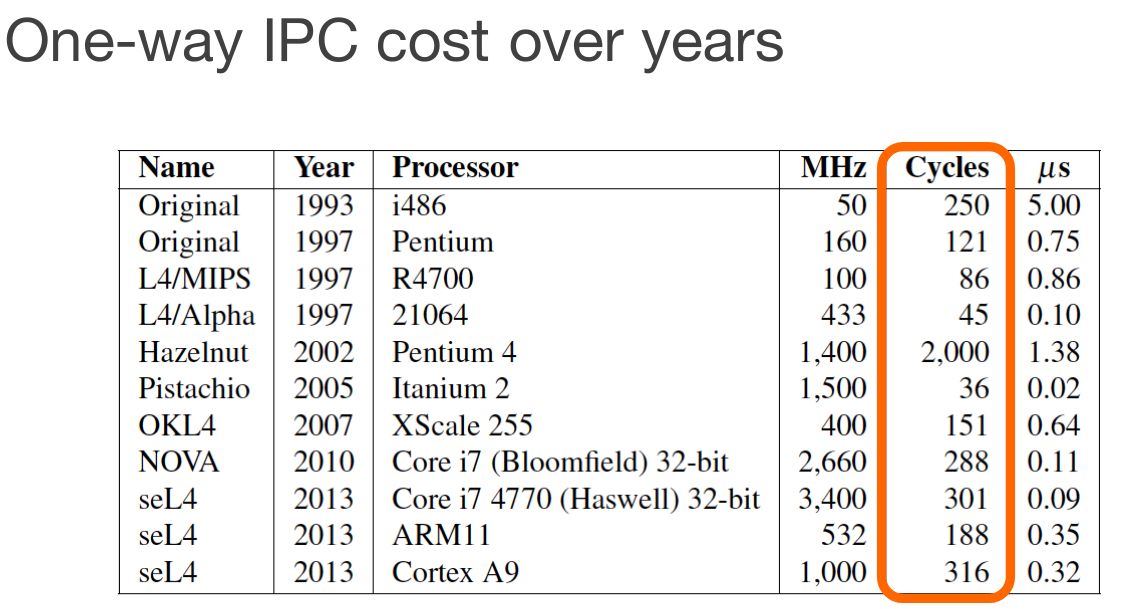
\includegraphics[width=.8\textwidth]{l4-ipc-perf}
	
\end{frame}

%https://ucbrise.github.io/cs262a-spring2018/notes/18-microkerenels-Mach-seL4.pdf
%-------------------------------------------------
\begin{frame}[plain]
	\frametitle{L4 family}
	
	\centering
	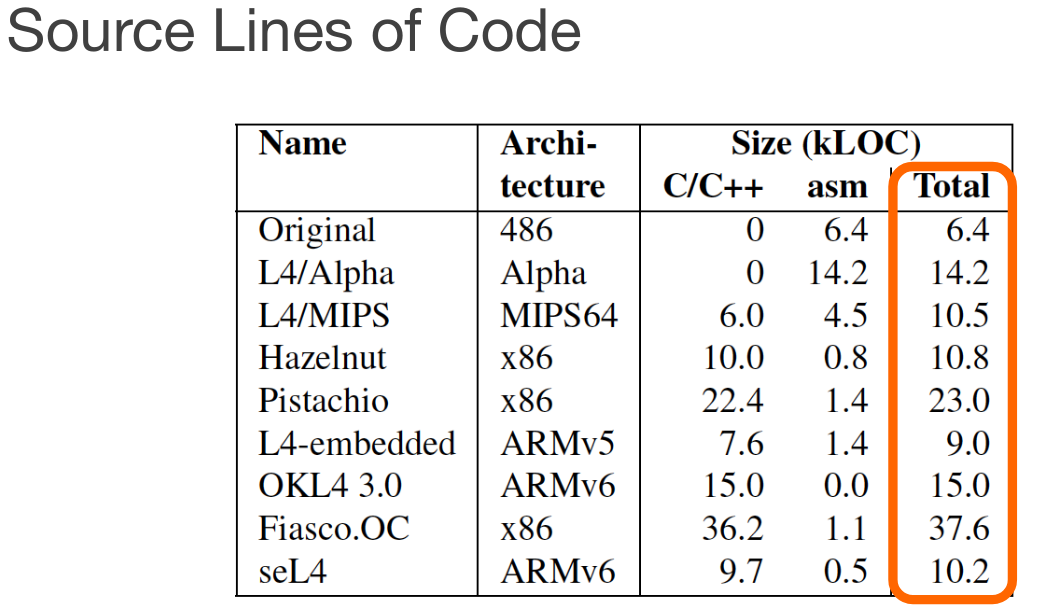
\includegraphics[width=.8\textwidth]{l4-src-code}
	
\end{frame}
%-------------------------------------------------


\end{document}